\documentclass[10pt,twocolumn]{article}
\usepackage[margin=0.7in]{geometry}
\usepackage{times}
\usepackage{amsmath,amssymb,amsthm}
\usepackage{booktabs,graphicx,hyperref,microtype}
\usepackage[numbers]{natbib}
\setlength{\parskip}{0.15em}
\setlength{\parindent}{1em}
\newtheorem{proposition}{Proposition}
\newtheorem{theorem}{Theorem}
\newcommand{\cFP}{c_{\mathrm{FP}}}
\newcommand{\cFN}{c_{\mathrm{FN}}}
\newcommand{\cE}{c_{E}}
\title{\vspace{-1.2em}\textbf{RiskTriage: Risk-Averse Calibration\\for Simulation-to-Experiment Catalyst Decisions}\vspace{-0.6em}}
\author{Anonymous authors\\Workshop paper (4 pages)}
\date{}
\begin{document}
\maketitle
\vspace{-1.2em}
\begin{abstract}
\vspace{-0.3em}
Computational screening produces uncertain catalyst recommendations, but physical validation is costly. We formulate translation as a \emph{risk-sensitive sequential decision}: whether to synthesize, characterize, electrochemically test, or reject a computational candidate. On Open Catalyst Experiments 2024 (OCx24) HER, a LightGBM predictor of cell voltage at \(50\,\mathrm{mA\,cm^{-2}}\) attains leave-one-composition-out \(R^2{=}0.61\): useful signal with enough residual uncertainty that triage matters. Calibrating nested prediction sets to a catalyst-specific decision loss, rather than to generic coverage, yields the operational quantity \(T(r)=\min P(\mathrm{TEST})\) subject to decision risk \(R\le r\). At \(R\le 0.10\), RiskTriage requires \textbf{8.4\%} {[4.2,\,13.4]} physical tests versus \textbf{16.5\%} {[9.2,\,24.4]} for uncertainty sampling and \textbf{25.9\%} {[22.3,\,29.6]} for split conformal (20 grouped seeds; bootstrap 95\% CI). Under composition shift the same policy becomes more conservative (\(7\%\to 21\%\) tests). Interval max-min rules are insensitive to experimental cost \(c_E\) until the Bayes testing region empties; cost-aware Bayes thresholds \emph{do} shut off testing at the theoretical cap \(c_E\ge \cFP\cFN/(\cFP+\cFN)\).
\vspace{-0.4em}
\end{abstract}

\vspace{-0.5em}
\section{Introduction}
\vspace{-0.3em}
The translational bottleneck in computational catalysis is not a missing predictor. It is a \emph{decision}: given an uncertain computational score, should a laboratory spend synthesis, X-ray characterization, and electrolysis on this candidate? Ordinary conformal prediction answers a different question---what interval covers \(Y\) with probability \(1-\alpha\)---and can force almost every candidate into the experimental queue. Risk-averse calibration~\citep{kiyani2025} and conformal risk control~\citep{angelopoulos2024crc} instead attach uncertainty sets to a downstream loss.

We study hydrogen evolution on OCx24~\citep{abed2024ocx24}, whose experimental campaign was a funnel (targeted synthesis, XRF/XRD filtering, prioritized electrolysis), not a uniform reveal of labels. The paper claim is:
\begin{quote}
\vspace{-0.25em}
\emph{Decision-calibrated uncertainty beats prediction-calibrated uncertainty for experimentally relevant outcomes: at a fixed tolerance for wrong TRUST/DROP actions, fewer physical tests recover the same scientific risk budget.}
\vspace{-0.25em}
\end{quote}
We do \emph{not} claim a new conformal theorem, a GNN, or that RiskTriage dominates ranking for discovery. The contribution is a decision layer between screening and the physical workflow (Figure~\ref{fig:main}a) and a matched-risk efficiency result (Figure~\ref{fig:main}b, Table~\ref{tab:main}).

\vspace{-0.4em}
\section{A three-action catalyst problem}
\vspace{-0.3em}
Let \(Y\) be experimental HER voltage vs.\ SHE at \(50\,\mathrm{mA\,cm^{-2}}\) (higher/less negative is better). Success is \(G=\mathbf{1}\{Y\ge y^\star\}\) with \(y^\star\) the training 75th percentile (\({\approx}{-}1.27\,\mathrm{V}\); 25\% positives). Actions \(a\in\{\mathrm{DROP},\mathrm{TEST},\mathrm{TRUST}\}\) incur
\[
L(\mathrm{TRUST},G)=\cFP(1-G),\quad
L(\mathrm{DROP},G)=\cFN G,\quad
L(\mathrm{TEST},G)=\cE.
\]
Triage risk \(R_{\mathrm{triage}}=\mathbb{E}[L]\) \emph{excluding} \(\cE\): TEST pays money, not a scientific misclassification. The operational program is
\begin{equation}
\min_{\lambda}\; \mathbb{E}[\mathbf{1}\{a_\lambda=\mathrm{TEST}\}]
\quad\text{s.t.}\quad
R_{\mathrm{triage}}(\lambda)\le r^\star.
\label{eq:program}
\end{equation}

\paragraph{When is TEST valuable?}
Let \(p(x)=P(G{=}1\mid x)\). Expected risks are \(R_T=(1-p)\cFP\), \(R_D=p\cFN\), \(R_E=\cE\).

\begin{proposition}[Bayes testing region]
If \(\cE < \cFP\cFN/(\cFP+\cFN)\), then
\(a^\star=\mathrm{DROP}\) for \(p\le \cE/\cFN\),
\(\mathrm{TRUST}\) for \(p\ge 1-\cE/\cFP\),
and \(\mathrm{TEST}\) in between. Otherwise TEST is never uniquely optimal.
\end{proposition}
\vspace{-0.35em}
\emph{Proof sketch.} TEST beats DROP iff \(p>\cE/\cFN\) and beats TRUST iff \(p<1-\cE/\cFP\). The interval is nonempty iff the displayed cap holds. \(\square\)

Value of a perfect experiment is \(\mathrm{VOI}(x)=\min\{p\cFN,(1-p)\cFP\}\); TEST iff \(\mathrm{VOI}>\cE\), recovering the same interval. Variance sampling does not:
\begin{proposition}[Uncertainty \(\neq\) VOI]
There exist \(x_1,x_2\) with \(\mathrm{Var}(Y\mid x_1)>\mathrm{Var}(Y\mid x_2)\) but \(\mathrm{VOI}(x_1)<\mathrm{VOI}(x_2)\).
\end{proposition}
\vspace{-0.35em}
A law supported on \(\{-100,-1\}\) can have arbitrary variance and \(P(Y\ge 0)=0\), hence \(\mathrm{VOI}=0\); a balanced \(\{\pm 1\}\) law has modest variance and \(\mathrm{VOI}=1/2\) under unit costs.

\paragraph{Sets to actions.}
Given \(C(x)=[L(x),U(x)]\),
\begin{equation}
a(x)=\begin{cases}
\mathrm{TRUST} & L(x)\ge y^\star,\\
\mathrm{DROP} & U(x)< y^\star,\\
\mathrm{TEST} & \text{otherwise.}
\end{cases}
\label{eq:interval}
\end{equation}
\begin{theorem}[Wrong non-test \(\subseteq\) noncoverage]
If \(P(Y\in C(X))\ge 1-\alpha\), then \(P(\text{wrong TRUST or DROP})\le \alpha\).
\end{theorem}
\vspace{-0.35em}
A wrong TRUST implies \(Y<y^\star\le L(X)\); a wrong DROP implies \(Y\ge y^\star>U(X)\). Both sit in \(\{Y\notin C(X)\}\). This is a catalyst-specific corollary of ordinary conformal validity, not a new coverage theorem.

The max-min (RAC) action \(a_C=\arg\max_a\inf_{y\in C} u(a,y)\) with \(u=-L\) coincides with~\eqref{eq:interval} whenever \(\cE<\min(\cFP,\cFN)\): on a straddling interval the worst-case utilities of TRUST and DROP are \(-\cFP,-\cFN\), so TEST wins. Hence for our default costs \((\cFP,\cFN,\cE)=(1,1,0.2)\), RAC and conformal risk control on nested residual sets are the same finite-sample rule: smallest \(\lambda\) such that
\(\frac{n}{n+1}\widehat R_n(\lambda)+\frac{B}{n+1}\le r^\star\)
with \(B=\max(\cFP,\cFN)\)~\citep{angelopoulos2024crc,kiyani2025}. Cost \(c_E\) enters Bayes thresholds (Prop.~1), not this max-min interval rule, until the testing region is empty.

\paragraph{Characterization as information.}
With XRF/XRD features \(Z\), \(V(X)=\max_a\mathbb{E}[u(a,Y)\mid X]\) and \(V(X,Z)=\max_a\mathbb{E}[u\mid X,Z]\) satisfy \(\mathbb{E}[V(X,Z)\mid X]\ge V(X)\) by the tower property (optionality of \(Z\)). The empirical question is how much electrochemical testing \(Z\) avoids.

\vspace{-0.4em}
\section{OCx24 HER protocol}
\vspace{-0.3em}
We use the public OCx24 joined HER table (179 experimental targets, all at \(50\,\mathrm{mA\,cm^{-2}}\); 166 sample IDs; 45 alloy families; 43 XRD-matched)~\citep{abed2024ocx24}. Features: mean/Wulff/Boltzmann adsorption energies for \(\{\mathrm{H},\mathrm{OH},\mathrm{CO},\mathrm{C},\mathrm{CHO},\mathrm{COCOH}\}\) plus composition descriptors (period, group, mass, radius, electronegativity, Mendeleev number). No GNN, no new DFT. Predictors: linear, ridge, random forest, LightGBM; a 5-member LightGBM ensemble supplies a scale for nested sets \(C_\lambda(x)=[\hat y\pm\lambda\,\sigma(x)]\).

Splits group replicate SIDs (65/17.5/17.5 train/cal/test). OOD holds out composition clusters. We report 20 seeds. Success threshold \(y^\star\) is fit on train only. Default \(r^\star{=}0.15\) in the CRC bound; matched-risk tables sweep realized test-set triage risk.

\vspace{-0.4em}
\section{Results}
\vspace{-0.3em}
\paragraph{Prediction fidelity and risk-efficient physical validation.}
The LightGBM base predictor achieves $R^2{=}0.605$, MAE ${=}0.079\,\mathrm{V}$, and Spearman ${=}0.791$ (Table~\ref{tab:main}a), reproducing the ${\sim}0.59$--$0.61$ HER signal reported for OCx24~\citep{abed2024ocx24}. Computational screening is therefore informative, but sufficiently imperfect for physical validation to remain relevant. Our primary endpoint is the minimum physical-testing fraction $T(r)=\min_{\pi:R(\pi)\le r}\Pr_\pi(\mathrm{TEST})$. At $R\le 0.10$, RAC/CRC requires only $8.4\%$ {[4.2,\,13.4]} of candidates to be tested, versus $16.5\%$ {[9.2,\,24.4]} for uncertainty sampling and $25.9\%$ {[22.3,\,29.6]} for split conformal (Table~\ref{tab:main}b; Figure~\ref{fig:main}). Thus calibrating uncertainty to downstream decision risk approximately halves physical validation relative to uncertainty sampling at this operating point. Linear, ridge, and random-forest leave-one-composition-out $R^2$ are $0.52$, $0.56$, and $0.60$.

\begin{figure}[t]
\centering
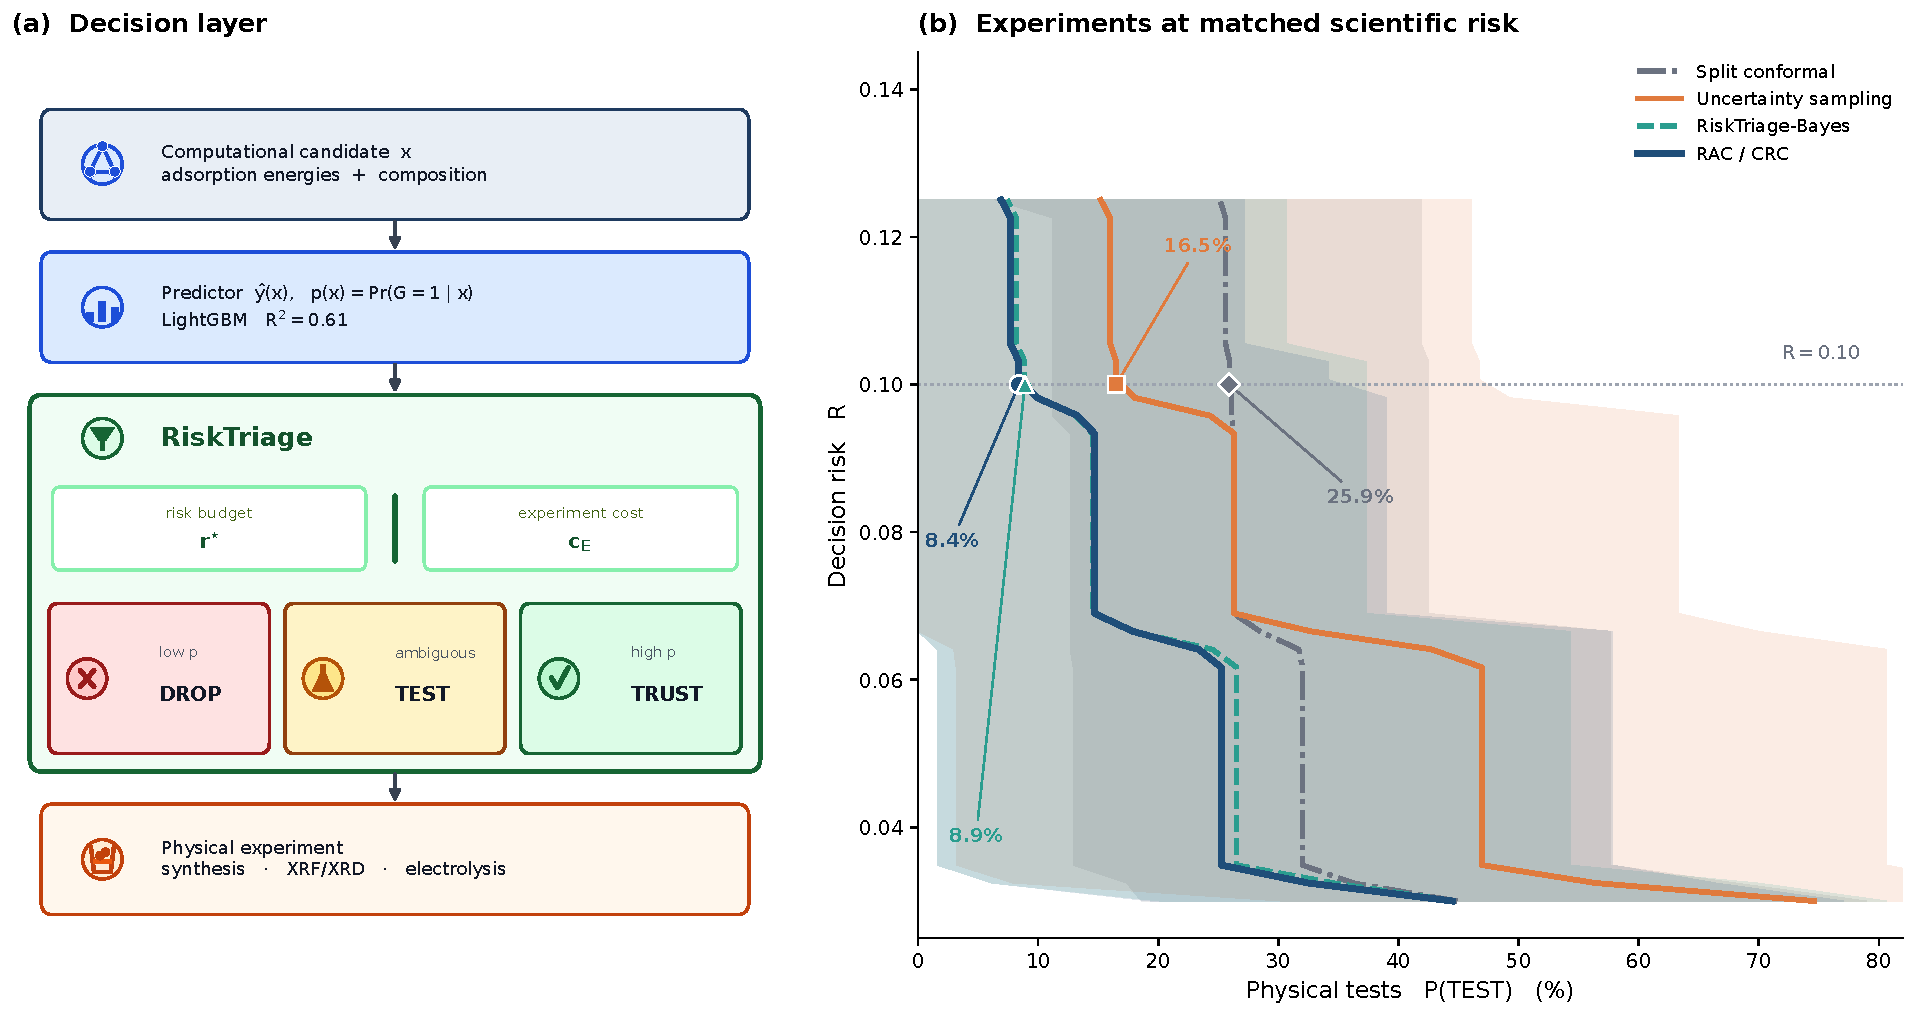
\includegraphics[width=\linewidth]{figures/fig1_risktriage.pdf}
\caption{\textbf{RiskTriage as a lab decision layer.}
\textbf{(a)}~A computational candidate is mapped to $p(x)=\Pr(G{=}1\mid x)$; RiskTriage chooses DROP / TEST / TRUST from a risk budget $r^\star$ and experimental cost $c_E$.
\textbf{(b)}~Pareto frontier of physical-testing rate versus decision risk (mean and 2.5--97.5\% seed band, 20 grouped splits). The $R{=}0.10$ operating point is marked: RAC/CRC $8.4\%$, RiskTriage-Bayes $8.9\%$, uncertainty sampling $16.5\%$, split conformal $25.9\%$. Lower-left is better.}
\label{fig:main}
\end{figure}

\begin{table}[t]
\centering
\caption{\textbf{Prediction fidelity and experimental efficiency.}
Top: the deployed predictor reproduces the OCx24 HER simulation-to-experiment signal.
Bottom: minimum fraction of candidates (\%) requiring physical testing at matched decision risk (bootstrap 95\% CIs, 20 grouped splits).}
\label{tab:main}
\small
\setlength{\tabcolsep}{3.5pt}
{\small
\begin{tabular}{lcccc}
\toprule
\multicolumn{5}{c}{\textbf{(a) Base predictor}}\\
\midrule
Model & $R^2$ & MAE & RMSE & Spearman \\
\midrule
LightGBM & 0.605 & 0.079 & 0.101 & 0.791 \\
\midrule
\multicolumn{5}{c}{\textbf{(b) Physical testing required at matched decision risk}}\\
\midrule
Max risk $r$ & RAC/CRC & RiskTriage-Bayes & Uncertainty & Split CP \\
\midrule
0.03  & 44.5 [36.9, 53.1] & 44.7 [36.7, 53.9] & 74.6 [65.2, 82.5] & 44.9 [37.0, 53.2] \\
0.05  & \textbf{25.2 [18.3, 32.6]} & 26.5 [19.3, 33.9] & 47.0 [35.3, 58.0] & 32.0 [26.8, 37.4] \\
0.075 & 14.7 [9.3, 20.5] & \textbf{14.5 [9.2, 20.1]} & 26.3 [16.4, 36.5] & 26.3 [22.7, 29.8] \\
\textbf{0.10} & \textbf{8.4 [4.2, 13.4]} & 8.9 [4.3, 14.3] & 16.5 [9.2, 24.4] & 25.9 [22.3, 29.6] \\
0.125 & \textbf{6.9 [3.3, 11.2]} & 7.4 [3.4, 12.2] & 15.2 [8.1, 22.9] & 25.1 [21.1, 28.9] \\
\bottomrule
\end{tabular}}
\end{table}

Split conformal at $\alpha{=}0.1$ covers $Y$ at rate $0.94$ with almost no wrong TRUST/DROP actions, yet sends ${\sim}75\%$ of candidates to TEST---statistically safe, experimentally inefficient. Reverse frontier: at a 10\% testing budget, RAC/CRC risk is $0.096$ {[0.074,\,0.122]} versus $0.113$ {[0.086,\,0.142]} for uncertainty sampling. Discovery AUDC is essentially unchanged versus LightGBM rank ($0.929$ vs.\ $0.927$; paired $\Delta{=}0.002$ {[0.000,\,0.006]})---RiskTriage's gain is safe abstention, not ranking.

\paragraph{Characterization, OOD, and cost.}
Updating the predictor with XRF/XRD features lowers TEST rate $7.4\%\to 5.1\%$ with a small risk increase ($0.114\to 0.125$). Hard-dropping XRD-unmatched materials before electrolysis cuts tests to $1.1\%$ but raises risk to $0.146$ and loses good catalysts (${\approx}2\%$ of the pool). Holding out alloy families, RAC TEST rate rises $7.4\%\to 21\%$ ($2.9\times$); split CP stays high ($75\%\to 81\%$). Sweeping $\cE\in\{0.01,\ldots,0.8\}$: Bayes $P(\mathrm{TEST})$ falls $5.9\%\to 0\%$ and is exactly $0$ for $\cE\ge 1/2$ (Prop.~1). Interval max-min RAC stays at $7.4\%$ for all $\cE\le 0.8<1$. Treat interval RAC as \emph{risk}-calibrated, not \emph{cost}-calibrated, unless Bayes thresholds are used.

\vspace{-0.4em}
\section{Limitations}
\vspace{-0.3em}
\(n{=}179\) labeled HER targets; CIs on \(T(0.10)\) are wide. Labels are not a logging policy over the 19k computational candidates; we do not claim off-policy optimality (IPW on XRD-match as a coarse propensity does not change MAE). RAC\(\equiv\)CRC for this three-action utility. CO\(_2\)RR is left to future work. Replicate noise in OCx24 is \({\sim}0.043\,\mathrm{V}\); our MAE \(0.079\,\mathrm{V}\) is above that floor.

\vspace{-0.4em}
\section{Conclusion}
\vspace{-0.3em}
Uncertainty for catalyst translation should be calibrated to the physical decision it controls. On OCx24 HER, nested-set risk control achieves a given scientific error tolerance with substantially fewer electrochemical tests than coverage conformalization or variance sampling, becomes more conservative under composition shift, and does not automatically improve top-decile discovery over predicted-performance ranking.

{\small
\bibliographystyle{plainnat}
\begin{thebibliography}{9}
\bibitem[Abed et~al.(2024)]{abed2024ocx24}
J.~Abed et~al.
\newblock Open Catalyst Experiments 2024 (OCx24).
\newblock arXiv:2411.11783, 2024.
\bibitem[Angelopoulos et~al.(2024)]{angelopoulos2024crc}
A.~N. Angelopoulos, S.~Bates, A.~Fisch, L.~Lei, and T.~Zrnic.
\newblock Conformal risk control.
\newblock \emph{ICLR}, 2024.
\bibitem[Kiyani et~al.(2025)]{kiyani2025}
S.~Kiyani, G.~Pappas, A.~Roth, and H.~Hassani.
\newblock Decision theoretic foundations for conformal prediction.
\newblock \emph{ICML}, 2025.
\end{thebibliography}
}
\end{document}
